\chapter{बफ़र और प्रभाविता आरेख}\label{ch:g12:buffers-predominance}

रक्त की एक जाँच धमनी-रक्त का \omterm{def:g9:acids-bases-ph:ph}{pH} बताती है: सामान्यतः 7.38 और
7.42 के बीच। काम करती पेशियाँ रक्त में अम्ल उड़ेलती हैं, फेफड़े उससे कार्बन
डाइऑक्साइड बाहर निकालते हैं, भोजन अम्ल और क्षारक लाता है; फिर भी \omterm{def:g9:acids-bases-ph:ph}{pH} मुश्किल से
हिलता है। स्पीशीज़ का एक जोड़ा, एक अम्ल और उसका अपना क्षारक, इन झटकों को सोख लेता है।
यह अध्याय दिखाता है कि किसी दिए गए \omterm{def:g9:acids-bases-ph:ph}{pH} पर किसी युग्म का कौन-सा रूप प्रभावी होता है, किसी
रंगीन युग्म की कुछ बूँदें \omterm{def:g9:acids-bases-ph:ph}{pH} को कैसे प्रकट करती हैं, और किसी
अम्ल और उसके क्षारक का \omterm{def:g6:pure-substances-and-mixtures:mixture}{मिश्रण} \omterm{def:g9:acids-bases-ph:ph}{pH} को कैसे स्थिर रखता है।

\begin{recall}
\omterm{def:g12:ka-and-pka:bronsted}{अम्ल--क्षारक युग्म}, $K_a$ और $pK_a$; किसी विलयन का \omterm{def:g9:acids-bases-ph:ph}{pH}
(\cref{ch:g12:ka-and-pka}, \cref{ch:g9:acids-bases-ph})।
\end{recall}

\begin{omfigure}
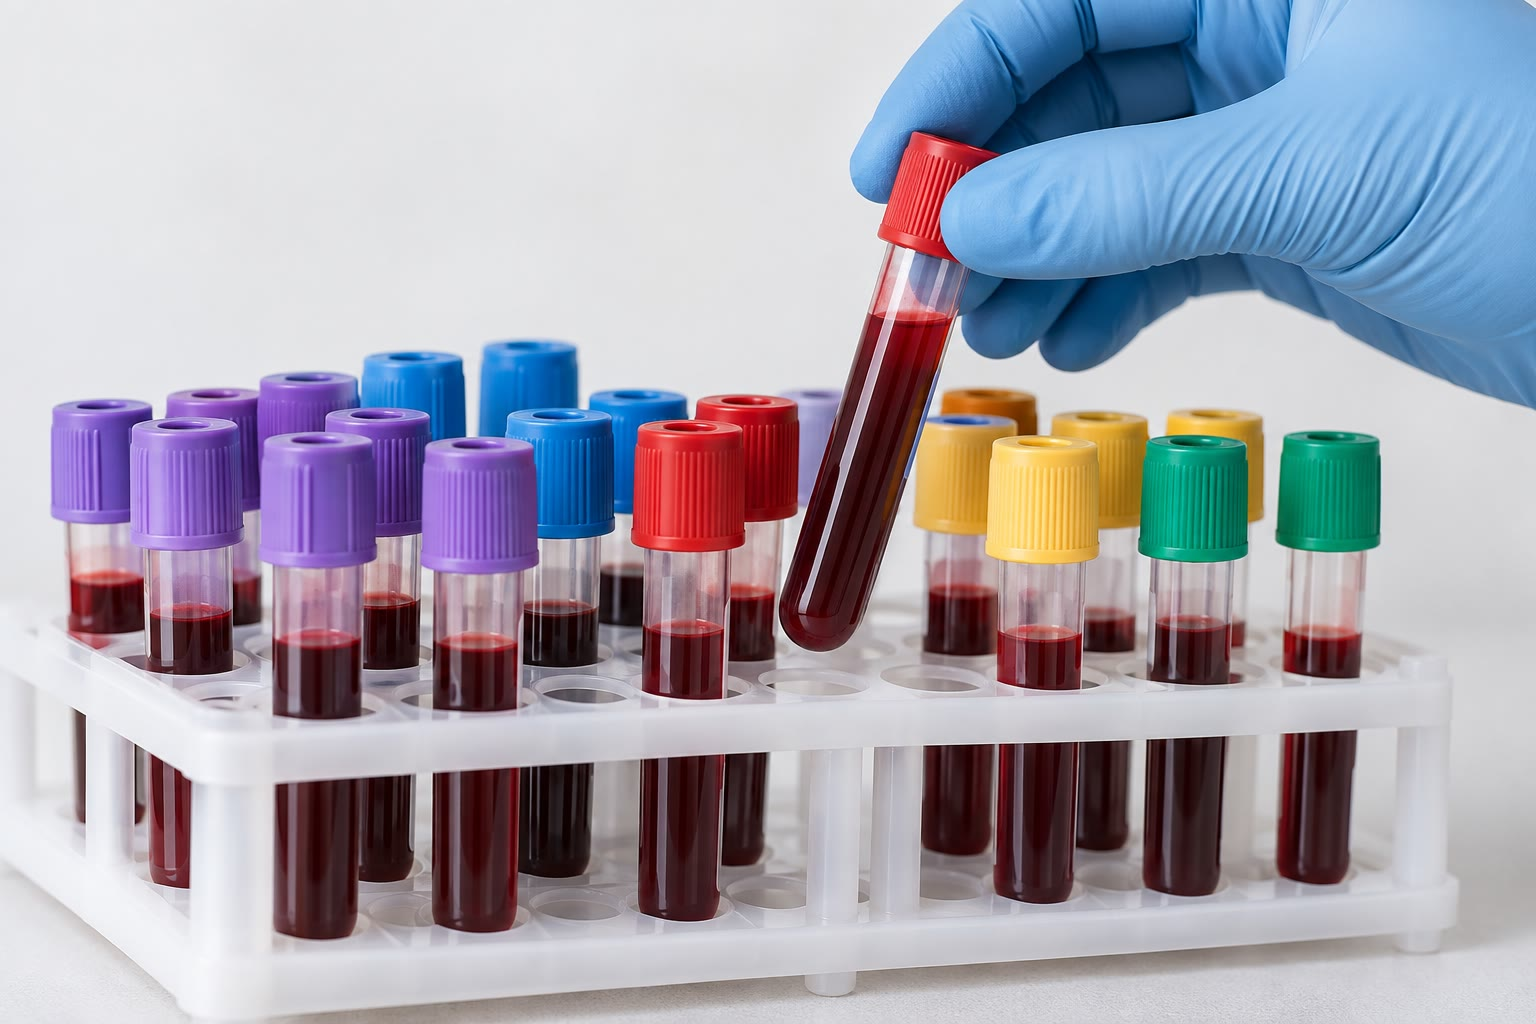
\includegraphics[width=0.45\linewidth]{images/book1/ai/g12-blood-tubes.jpg}

{\small रक्त के नमूने: उनका \omterm{def:g9:acids-bases-ph:ph}{pH} एक संकरे परास में बना रहता है।}
\end{omfigure}

\section{प्रभाविता आरेख}

\begin{proposition}[हेंडरसन संबंध]\label{prop:g12:buffers-predominance:henderson}
युग्म \ce{HA}/\ce{A-} वाले किसी भी \omterm{def:g6:solutions-and-solubility:solute}{जलीय विलयन} में,
\[
  \mathrm{pH} = pK_a + \log\frac{[\ce{A-}]}{[\ce{HA}]} .
\]
\end{proposition}

\begin{proof}
$K_a = \dfrac{[\ce{A-}][\ce{H3O+}]}{[\ce{HA}]c^\circ}$ से, दोनों पक्षों का $-\log$
लीजिए: $pK_a = \mathrm{pH} - \log\dfrac{[\ce{A-}]}{[\ce{HA}]}$।
\end{proof}

\begin{definition}[प्रभाविता और वितरण आरेख]\label{def:g12:buffers-predominance:predominance}
किसी युग्म का \emph{प्रभाविता आरेख}\index{प्रभाविता आरेख}
$pK_a$ पर विभाजित एक \omterm{def:g9:acids-bases-ph:ph}{pH} अक्ष है: उसके नीचे अम्ल HA प्रभावी होता है
($[\ce{HA}] > [\ce{A-}]$), ऊपर क्षारक \ce{A-}। \emph{वितरण
आरेख}\index{वितरण आरेख} \omterm{def:g9:acids-bases-ph:ph}{pH} के विरुद्ध हर रूप का अंश,
$[\ce{HA}]/c$ और $[\ce{A-}]/c$, दिखाता है; दोनों वक्र
$\mathrm{pH} = pK_a$ पर एक-दूसरे को काटते हैं।
\end{definition}

\begin{method}[प्रभाविता आरेख बनाना]\label{met:g12:buffers-predominance:diagram}
\begin{enumerate}
  \item 0 से 14 तक एक \omterm{def:g9:acids-bases-ph:ph}{pH} अक्ष बनाइए और युग्म का $pK_a$ चिह्नित कीजिए।
  \item अम्ल को $pK_a$ के बाईं ओर और क्षारक को दाईं ओर लिखिए।
  \item कई युग्मों वाली स्पीशीज़ (देने के लिए दो हाइड्रोजन वाला अम्ल,
        कोई ऐमीनो अम्ल) के लिए हर $pK_a$ चिह्नित कीजिए: हर अंतराल
        एक रूप का होता है।
  \item $pK_a$ से एक इकाई दूर ही अनुपात 10 और 1 का हो जाता है: अल्प
        रूप \qty{10}{\percent} से कम होता है।
\end{enumerate}
\end{method}

\begin{omfigure}
\begin{tikzpicture}[font=\small, x=0.62cm]
  % ledger: pka:ethanoic, pka:methanoic, kb:NH3, ka:H2CO3
  \foreach \y/\pk/\acid/\base in {0/3.74/{\ce{HCOOH}}/{\ce{HCOO-}},
      -1.0/4.76/{\ce{CH3COOH}}/{\ce{CH3COO-}}, -2.0/6.37/{\ce{CO2,H2O}}/{\ce{HCO3-}},
      -3.0/9.26/{\ce{NH4+}}/{\ce{NH3}}} {
    \fill[omThm!20] (0,\y) rectangle (\pk,\y+0.5);
    \fill[omDef!20] (\pk,\y) rectangle (14,\y+0.5);
    \draw[black!50] (0,\y) rectangle (14,\y+0.5);
    \node at (\pk/2,\y+0.25) {\acid};
    \node at ({(\pk+14)/2},\y+0.25) {\base};
    \draw[thick] (\pk,\y-0.08) -- (\pk,\y+0.58);
    \node[font=\scriptsize, anchor=south] at (\pk,\y+0.55) {\pk};
  }
  \draw[->] (0,-3.4) -- (14.5,-3.4) node[right] {pH};
  \foreach \k in {0,2,4,6,8,10,12,14} \draw (\k,-3.35) -- (\k,-3.45) node[below, font=\scriptsize] {\k};
\end{tikzpicture}

{\small चार युग्मों के \omterm{def:g12:buffers-predominance:predominance}{प्रभाविता आरेख}: अम्ल (बाएँ, लाल) अपने $pK_a$ से नीचे
प्रभावी होता है, क्षारक (दाएँ, नीला) उससे ऊपर।}
\end{omfigure}

\begin{omfigure}
\begin{minipage}{0.49\linewidth}
\begin{tikzpicture}
\begin{axis}[width=\linewidth, height=5cm, xmin=0, xmax=14, ymin=0, ymax=1.05,
    xlabel={pH}, ylabel={अंश}, axis lines*=left, ymajorgrids,
    grid style={gray!20}, tick label style={font=\scriptsize},
    label style={font=\small}, title={\small एथेनोइक अम्ल},
    title style={yshift=-4pt}]
  \addplot[very thick, omThm] table[x=pH, y=HA] {figdata/out/grade-12-buffers-predominance-a.dat};
  \addplot[very thick, omDef] table[x=pH, y=A] {figdata/out/grade-12-buffers-predominance-a.dat};
  \addplot[dashed, black!50] coordinates {(4.76,0) (4.76,1)};
  \node[font=\scriptsize, omThm] at (axis cs:2.2,0.85) {\ce{CH3COOH}};
  \node[font=\scriptsize, omDef] at (axis cs:7.6,0.85) {\ce{CH3COO-}};
\end{axis}
\end{tikzpicture}
\end{minipage}\hfill
\begin{minipage}{0.49\linewidth}
\begin{tikzpicture}
\begin{axis}[width=\linewidth, height=5cm, xmin=0, xmax=14, ymin=0, ymax=1.05,
    xlabel={pH}, ylabel={अंश}, axis lines*=left, ymajorgrids,
    grid style={gray!20}, tick label style={font=\scriptsize},
    label style={font=\small}, title={\small ग्लाइसीन},
    title style={yshift=-4pt}]
  \addplot[very thick, omThm] table[x=pH, y=cation] {figdata/out/grade-12-buffers-predominance-b.dat};
  \addplot[very thick, omMeth] table[x=pH, y=zwitterion] {figdata/out/grade-12-buffers-predominance-b.dat};
  \addplot[very thick, omDef] table[x=pH, y=anion] {figdata/out/grade-12-buffers-predominance-b.dat};
  \node[font=\scriptsize, omThm] at (axis cs:1.0,0.55) {धनायन};
  \node[font=\scriptsize, omMeth] at (axis cs:6.1,0.88) {ज़्विटर आयन};
  \node[font=\scriptsize, omDef] at (axis cs:12.6,0.55) {ऋणायन};
\end{axis}
\end{tikzpicture}
\end{minipage}

{\small $pK_a$ मानों से निकाले गए \omterm{def:g12:buffers-predominance:predominance}{वितरण आरेख}। बाएँ:
एथेनोइक अम्ल, वक्र 4.76 पर काटते हैं। दाएँ: ग्लाइसीन,
\ce{H2N-CH2-COOH}, दो युग्मों के साथ ($pK_a$ 2.35 और 9.78): \omterm{def:g9:ions:ion}{धनायन}
\ce{H3N+-CH2-COOH}, ज़्विटर \omterm{def:g9:ions:ion}{आयन} \ce{H3N+-CH2-COO-} और \omterm{def:g9:ions:ion}{ऋणायन}
\ce{H2N-CH2-COO-}।}
\end{omfigure}

\begin{example}[शरीर में ग्लाइसीन]\label{ex:g12:buffers-predominance:glycine}
% ledger: pka:glycine1, pka:glycine2, ph:blood
रक्त के \omterm{def:g9:acids-bases-ph:ph}{pH}, लगभग 7.4, पर ग्लाइसीन अपने दोनों $pK_a$
मानों के बीच होता है: वह लगभग पूरी तरह ज़्विटर \omterm{def:g9:ions:ion}{आयन} रूप में होता है, जिसके
नाइट्रोजन पर धनात्मक आवेश और कार्बोक्सिलेट पर ऋणात्मक आवेश होता है,
और कुल मिलाकर वह उदासीन होता है। हर ऐमीनो अम्ल इसी तरह व्यवहार करता है।
\end{example}

\section{अम्ल--क्षारक सूचक}


\begin{definition}[अम्ल--क्षारक सूचक, रंग-परिवर्तन परास]\label{def:g12:buffers-predominance:indicator}
\emph{अम्ल--क्षारक सूचक}\index{अम्ल--क्षारक सूचक} एक युग्म
\ce{HInd}/\ce{Ind-} है जिसके दोनों रूपों के रंग भिन्न होते हैं, और जिसे बहुत
थोड़ी मात्रा में इस्तेमाल किया जाता है। उसका \emph{रंग-परिवर्तन परास}\index{रंग-परिवर्तन परास}
वह \omterm{def:g9:acids-bases-ph:ph}{pH} अंतराल है जिस पर रंग बदलता दिखता है, मोटे तौर पर
$pK_a - 1$ से $pK_a + 1$ तक: उसके नीचे \ce{HInd} का रंग दिखता है, ऊपर
\ce{Ind-} का, और बीच में दोनों का \omterm{def:g6:pure-substances-and-mixtures:mixture}{मिश्रण}।
\end{definition}

\begin{omfigure}
\begin{tikzpicture}[font=\small, x=0.62cm]
  % ledger: ind:methyl-red, ind:BBT, ind:phenolphthalein, ind:thymol-blue, ind:range-rule
  \foreach \y/\name/\a/\b/\ca/\cm/\cb in {
      0/{मेथिल रेड}/4.2/6.3/red!70/orange/yellow!80,
      -0.8/{ब्रोमोथाइमॉल ब्लू}/6.0/7.6/yellow!80/green!60/blue!60,
      -1.6/{फ़ीनॉल्फ़्थेलीन}/8.0/10.0/white/magenta!25/magenta!70} {
    \fill[\ca] (0,\y) rectangle (\a,\y+0.5);
    \shade[left color=\ca, right color=\cb] (\a,\y) rectangle (\b,\y+0.5);
    \fill[\cb] (\b,\y) rectangle (14,\y+0.5);
    \draw[black!50] (0,\y) rectangle (14,\y+0.5);
    \node[anchor=east] at (-0.2,\y+0.25) {\name};
  }
  \fill[red!65] (0,-2.4) rectangle (1.2,-1.9);
  \shade[left color=red!65, right color=yellow!80] (1.2,-2.4) rectangle (2.8,-1.9);
  \fill[yellow!80] (2.8,-2.4) rectangle (8.0,-1.9);
  \shade[left color=yellow!80, right color=blue!60] (8.0,-2.4) rectangle (9.1,-1.9);
  \fill[blue!60] (9.1,-2.4) rectangle (14,-1.9);
  \draw[black!50] (0,-2.4) rectangle (14,-1.9);
  \node[anchor=east] at (-0.2,-2.15) {थाइमॉल ब्लू};
  \draw[->] (0,-2.8) -- (14.5,-2.8) node[right] {pH};
  \foreach \k in {0,2,4,6,8,10,12,14} \draw (\k,-2.75) -- (\k,-2.85) node[below, font=\scriptsize] {\k};
\end{tikzpicture}

{\small \omterm{def:g9:acids-bases-ph:ph}{pH} के विरुद्ध चार सूचकों के रंग; छायांकित भाग
\omterm{def:g12:buffers-predominance:indicator}{रंग-परिवर्तन परास} हैं। थाइमॉल ब्लू, दो युग्मों के साथ, के दो
परास हैं।}
\end{omfigure}

\begin{method}[सूचक चुनना]\label{met:g12:buffers-predominance:indicator}
यह पता लगाने के लिए कि कोई विलयन किसी दिए गए \omterm{def:g9:acids-bases-ph:ph}{pH} को कब पार करता है (उदाहरण के लिए,
\omterm{def:g11:titration:titration}{अनुमापन} के अंत का \omterm{def:g9:acids-bases-ph:ph}{pH}), ऐसा सूचक चुनिए जिसके \omterm{def:g12:buffers-predominance:indicator}{रंग-परिवर्तन परास} में
वह \omterm{def:g9:acids-bases-ph:ph}{pH} हो: तब रंग ठीक वहीं बदलता है।
\end{method}

\section{बफ़र विलयन}

\begin{definition}[बफ़र विलयन]\label{def:g12:buffers-predominance:buffer}
\emph{बफ़र विलयन}\index{बफ़र विलयन} वह विलयन है जिसका \omterm{def:g9:acids-bases-ph:ph}{pH}
थोड़ा अम्ल या क्षारक मिलाने पर, या तनु करने पर, बहुत कम
बदलता है। यह आम तौर पर एक \omterm{def:g12:ka-and-pka:strong-acid}{दुर्बल अम्ल} और उसके संयुग्मी क्षारक की
तुलनीय मात्राओं से बना होता है; तब उसका \omterm{def:g9:acids-bases-ph:ph}{pH} युग्म के $pK_a$ के निकट होता है।
\end{definition}

\begin{proposition}[बफ़र प्रतिरोध क्यों करता है]\label{prop:g12:buffers-predominance:buffer}
\ce{HA} और \ce{A-} के बफ़र में, मिलाया गया \omterm{def:g12:ka-and-pka:strong-acid}{प्रबल अम्ल}
\ce{A-} द्वारा (\ce{A- + H3O+ -> HA + H2O}) और मिलाया गया \omterm{def:g12:ka-and-pka:strong-acid}{प्रबल क्षारक} \ce{HA} द्वारा
(\ce{HA + OH- -> A- + H2O}) खपा लिया जाता है; अनुपात $[\ce{A-}]/[\ce{HA}]$, और इसलिए
\omterm{def:g9:acids-bases-ph:ph}{pH}, केवल थोड़ा बदलता है। \omterm{def:g10:concentration-and-dilution:dilution}{तनुकरण} अनुपात को बिल्कुल नहीं बदलता।
\end{proposition}

\begin{proof}
हेंडरसन संबंध के अनुसार \omterm{def:g9:acids-bases-ph:ph}{pH} केवल अनुपात पर निर्भर करता है। हर रूप के
\qty{10}{mmol} वाले बफ़र में \qty{1}{mmol} अम्ल मिलाने से
अनुपात $10/10$ से $9/11$ हो जाता है, और \omterm{def:g9:acids-bases-ph:ph}{pH} केवल
$\log(9/11) = -0.09$ बदलता है।
\end{proof}

\begin{omfigure}
\begin{tikzpicture}
\begin{axis}[width=0.75\linewidth, height=5.6cm, xmin=0, xmax=10, ymin=0,
    ymax=8, xlabel={मिलाया गया \qty{0.10}{mol/L} का \ce{HCl} (\si{mL})},
    ylabel={pH}, axis lines*=left, ymajorgrids, grid style={gray!20},
    tick label style={font=\small}, label style={font=\small},
    legend style={font=\small, at={(0.98,0.97)}, anchor=north east,
    draw=none, fill=white}, legend cell align=left]
  % ledger: pka:ethanoic (buffer recipe: exercise data)
  \addplot[very thick, omThm, mark=*, mark size=1.3pt] table[x=V, y=water]
    {figdata/out/grade-12-buffers-predominance-c.dat};
  \addplot[very thick, omDef, mark=*, mark size=1.3pt] table[x=V, y=buffer]
    {figdata/out/grade-12-buffers-predominance-c.dat};
  \legend{\qty{100}{mL} शुद्ध पानी, \qty{100}{mL} एथेनोएट बफ़र}
\end{axis}
\end{tikzpicture}

{\small शुद्ध पानी में और एथेनोइक अम्ल और सोडियम एथेनोएट
(हर एक \qty{0.10}{mol/L}) के बफ़र में हाइड्रोक्लोरिक अम्ल \omterm{def:g2:mixing-and-dissolving:mix}{मिलाना}। पानी का \omterm{def:g9:acids-bases-ph:ph}{pH}
7 से लगभग 2 तक गिरता है; बफ़र का 4.76 से 4.67 तक।}
\end{omfigure}

\begin{method}[बफ़र तैयार करना]\label{met:g12:buffers-predominance:prepare}
\begin{enumerate}
  \item ऐसा युग्म चुनिए जिसका $pK_a$ वांछित \omterm{def:g9:acids-bases-ph:ph}{pH} से एक इकाई के भीतर हो
        (आदर्श रूप से उसके निकट)।
  \item अनुपात $[\ce{A-}]/[\ce{HA}] = 10^{\mathrm{pH} - pK_a}$ निकालिए।
  \item \omterm{def:g12:ka-and-pka:strong-acid}{दुर्बल अम्ल} और उसके क्षारक के किसी लवण को उस अनुपात में मिलाइए, ऐसी
        सांद्रताओं पर जो अम्ल या क्षारक की मात्राओं को सोखने के लिए
        पर्याप्त ऊँची हों।
\end{enumerate}
\end{method}

\begin{inthelab}[pH 4.8 पर बफ़र तैयार करना]
\qty{0.10}{mol/L} एथेनोइक अम्ल के \qty{50.0}{mL} को
\qty{0.10}{mol/L} सोडियम एथेनोएट के \qty{50.0}{mL} के साथ मिलाया जाता है; \omterm{def:g9:acids-bases-ph:ph-paper}{pH मीटर}
लगभग 4.8 पढ़ता है। \qty{1}{mol/L} हाइड्रोक्लोरिक अम्ल की कुछ बूँदें पाठ्यांक को
मुश्किल से हिलाती हैं, जबकि वही बूँदें \qty{100}{mL} आसुत जल में
उसे लगभग 3 तक गिरा देती हैं।
\end{inthelab}

\section{सजीवों में बफ़र}

\begin{example}[रक्त का बफ़र]\label{ex:g12:buffers-predominance:blood}
% ledger: pk:blood-bicarb, ph:blood, hco3:blood
रक्त का मुख्य बफ़र घुली हुई कार्बन डाइऑक्साइड और
हाइड्रोजनकार्बोनेट \omterm{def:g9:ions:ion}{आयन} का युग्म, \ce{CO2,H2O}/\ce{HCO3-}, है। रक्त में
शरीर-क्रिया विज्ञानी इसके लिए संबंध $\mathrm{pH} = 6.1 +
\log\big([\ce{HCO3-}]/[\ce{CO2}]\big)$ का उपयोग करते हैं। फेफड़े कार्बन डाइऑक्साइड हटाते हैं,
गुर्दे हाइड्रोजनकार्बोनेट को समायोजित करते हैं: मिलकर वे अनुपात को,
और इसलिए \omterm{def:g9:acids-bases-ph:ph}{pH} को, बनाए रखते हैं।
\end{example}

\begin{omfigure}
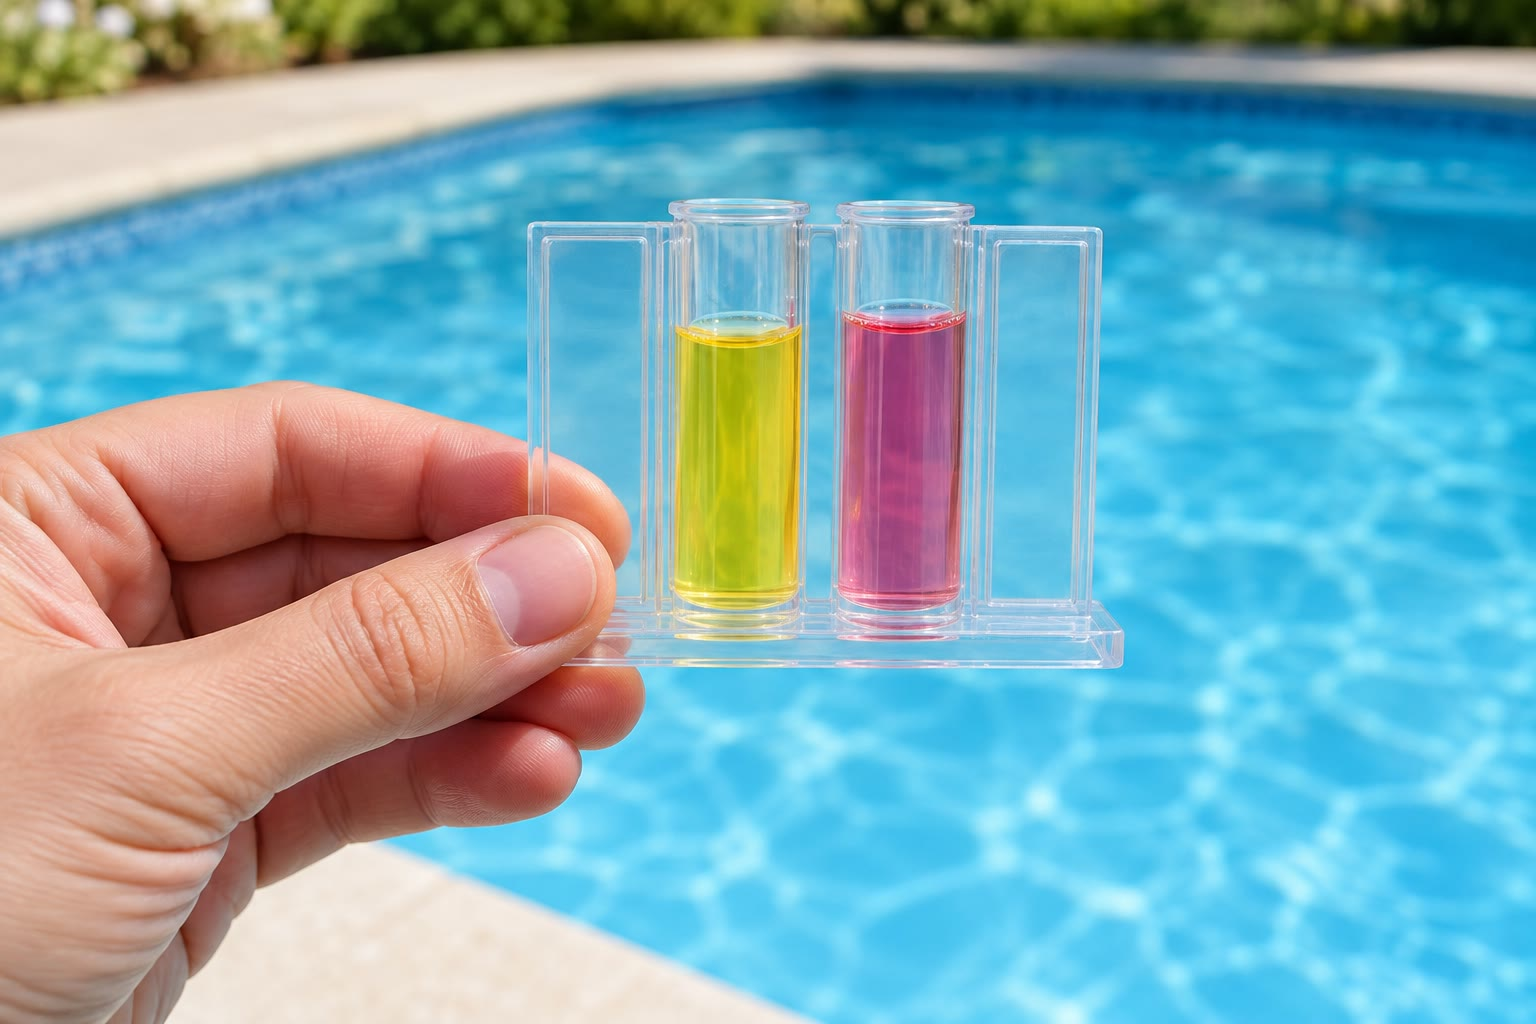
\includegraphics[width=0.45\linewidth]{images/book1/ai/g12-pool-test.jpg}

{\small स्विमिंग पूल के पानी की जाँच: सूचकों के रंग
\omterm{def:g9:acids-bases-ph:ph}{pH} बताते हैं।}
\end{omfigure}

\section{अभ्यास}


\begin{exercise}[$\star$]\label{exo:g12:buffers-predominance:1}
युग्म \ce{CH3COOH}/\ce{CH3COO-} ($pK_a = 4.76$) का कौन-सा रूप
\omterm{def:g9:acids-bases-ph:ph}{pH} 2, \omterm{def:g9:acids-bases-ph:ph}{pH} 4.76 और \omterm{def:g9:acids-bases-ph:ph}{pH} 7 पर प्रभावी होता है?
\end{exercise}

\begin{exercise}[$\star$]\label{exo:g12:buffers-predominance:2}
एथेनोइक अम्ल के \omterm{def:g12:buffers-predominance:predominance}{वितरण आरेख} पर \omterm{def:g9:acids-bases-ph:ph}{pH} 4 और \omterm{def:g9:acids-bases-ph:ph}{pH} 6 पर
\ce{CH3COO-} का अंश पढ़िए।
\end{exercise}

\begin{exercise}[$\star$]\label{exo:g12:buffers-predominance:3}
ब्रोमोथाइमॉल ब्लू \omterm{def:g9:acids-bases-ph:ph}{pH} 5 पर कौन-सा रंग दिखाता है? \omterm{def:g9:acids-bases-ph:ph}{pH} 7 पर? \omterm{def:g9:acids-bases-ph:ph}{pH} 9 पर?
\end{exercise}

\begin{exercise}[$\star$]\label{exo:g12:buffers-predominance:4}
\omterm{def:g9:acids-bases-ph:ph}{pH} 7.4 वाले विलयन में युग्म \ce{NH4+}/\ce{NH3} का कौन-सा रूप प्रभावी होता है?
\omterm{def:g9:acids-bases-ph:ph}{pH} 11 पर?
\end{exercise}

\begin{exercise}[$\star$]\label{exo:g12:buffers-predominance:5}
सूचक बहुत थोड़ी मात्रा में क्यों इस्तेमाल किए जाते हैं?
\end{exercise}

\begin{exercise}[$\star\star$]\label{exo:g12:buffers-predominance:6}
\omterm{def:g9:acids-bases-ph:ph}{pH} 3.76, 4.76 और 5.76 पर अनुपात $[\ce{CH3COO-}]/[\ce{CH3COOH}]$
निकालिए।
\end{exercise}

\begin{exercise}[$\star\star$]\label{exo:g12:buffers-predominance:7}
एक \omterm{def:g11:titration:titration}{अनुमापन} \omterm{def:g9:acids-bases-ph:ph}{pH} 8.7 पर समाप्त होता है। चित्र के चार सूचकों में से आप कौन-सा
चुनेंगे? मेथिल रेड क्यों नहीं?
\end{exercise}

\begin{exercise}[$\star\star$]\label{exo:g12:buffers-predominance:8}
एक बफ़र में \qty{0.20}{mol/L} एथेनोइक अम्ल और
\qty{0.10}{mol/L} सोडियम एथेनोएट है। उसका \omterm{def:g9:acids-bases-ph:ph}{pH} निकालिए।
\end{exercise}

\begin{exercise}[$\star\star$]\label{exo:g12:buffers-predominance:9}
ग्लाइसीन आरेख की मदद से \omterm{def:g9:acids-bases-ph:ph}{pH} 1, 6 और 12 पर प्रभावी रूप
उसके आवेश के साथ बताइए।
\end{exercise}

\begin{exercise}[$\star\star$]\label{exo:g12:buffers-predominance:10}
अनुक्रिया वक्र पढ़िए: \qty{1.0}{mL} अम्ल के बाद पानी का \omterm{def:g9:acids-bases-ph:ph}{pH} कितना
गिरता है? और बफ़र का?
\end{exercise}

\begin{exercise}[$\star\star$]\label{exo:g12:buffers-predominance:11}
\omterm{def:g9:acids-bases-ph:ph}{pH} 9.5 पर बफ़र बनाने के लिए आप प्रभाविता वाले चित्र का कौन-सा युग्म
चुनेंगे? उसके दोनों रूपों को आप किस अनुपात में मिलाएँगे?
\end{exercise}

\begin{exercise}[$\star\star\star$]\label{exo:g12:buffers-predominance:12}
चित्र वाले एथेनोएट बफ़र (हर रूप का \qty{10}{mmol}) में
हाइड्रोक्लोरिक अम्ल मिलाया जाता है। उसका \omterm{def:g9:acids-bases-ph:ph}{pH} एक इकाई गिरने से पहले वह कितना अम्ल
सह सकता है? अधिक सांद्र बफ़र की धारिता अधिक क्यों कही
जाती है?
\end{exercise}

\begin{exercise}[$\star\star\star$]\label{exo:g12:buffers-predominance:13}
\omterm{def:g9:acids-bases-ph:ph}{pH} 5.0 पर बफ़र पाने के लिए \qty{0.10}{mol/L} एथेनोइक अम्ल के \qty{100}{mL} में
\qty{0.10}{mol/L} सोडियम एथेनोएट विलयन का कितना आयतन मिलाना
चाहिए?
\end{exercise}

\begin{exercise}[$\star\star\star$]\label{exo:g12:buffers-predominance:14}
थाइमॉल ब्लू के दो \omterm{def:g12:buffers-predominance:indicator}{रंग-परिवर्तन परास} हैं। कारण समझाइए, और \omterm{def:g9:acids-bases-ph:ph}{pH} 1, 5 और 10 पर उसका
रंग बताइए।
\end{exercise}

\begin{exercise}[$\star\star\star$]\label{exo:g12:buffers-predominance:15}
\omterm{def:g9:acids-bases-ph:ph}{pH} 4.76 वाले एक बफ़र को आसुत जल से दस गुना तनु किया जाता है। हेंडरसन संबंध
के अनुसार उसका नया \omterm{def:g9:acids-bases-ph:ph}{pH} क्या है? यदि उसी \omterm{def:g9:acids-bases-ph:ph}{pH} वाले किसी \omterm{def:g12:ka-and-pka:strong-acid}{प्रबल
अम्ल} को दस गुना तनु किया जाए तो क्या होता है?
\end{exercise}

\section{समस्या: रक्त का बफ़र}

\begin{problem}[{सप्ताहांत समस्या --- हाइड्रोजनकार्बोनेट और
कार्बन डाइऑक्साइड का कौन-सा अनुपात रक्त को pH 7.4 पर रखता है?}]
\label{pb:g12:buffers-predominance:1}
% ledger: pk:blood-bicarb, ph:blood, hco3:blood
धमनी-रक्त का \omterm{def:g9:acids-bases-ph:ph}{pH} सामान्यतः 7.38 और 7.42 के बीच होता है। उसका मुख्य
बफ़र युग्म \ce{CO2,H2O}/\ce{HCO3-} है, जिसके लिए शरीर-क्रिया विज्ञानी
$\mathrm{pH} = 6.1 + \log\big([\ce{HCO3-}]/[\ce{CO2}]\big)$ का उपयोग करते हैं। रक्त में
हाइड्रोजनकार्बोनेट की सामान्य सांद्रता 22 से \qty{28}{mmol/L} होती है।

\medskip
\noindent\textbf{भाग I --- युग्म।}
\begin{enumerate}
  \item पानी के साथ घुली हुई कार्बन डाइऑक्साइड की वह अभिक्रिया लिखिए जो
        हाइड्रोजनकार्बोनेट \omterm{def:g9:ions:ion}{आयन} देती है।
  \item कौन-सी स्पीशीज़ अम्ल है, कौन-सी क्षारक?
  \item मान 6.1, $pK_a$ सारणी के 6.37 से भिन्न है। एक
        कारण बताइए (शरीर के ताप और मौजूद अन्य
        \omterm{def:g9:ions:ion}{आयनों} के बारे में सोचिए)।
  \item \qty{24}{mmol/L} पर \qty{5.0}{L} रक्त में हाइड्रोजनकार्बोनेट की कितनी मात्रा
        होती है?
\end{enumerate}

\medskip
\noindent\textbf{भाग II --- प्रभाविता।}
\begin{enumerate}[resume]
  \item $pK = 6.1$ के साथ युग्म का \omterm{def:g12:buffers-predominance:predominance}{प्रभाविता आरेख} बनाइए।
  \item रक्त में कौन-सा रूप प्रभावी है?
  \item रक्त थोड़ा अम्लीय है या थोड़ा क्षारकीय?
\end{enumerate}

\medskip
\noindent\textbf{भाग III --- अनुपात।}
\begin{enumerate}[resume]
  \item संबंध की मदद से \omterm{def:g9:acids-bases-ph:ph}{pH} 7.4 पर अनुपात $[\ce{HCO3-}]/[\ce{CO2}]$
        निकालिए।
  \item $[\ce{HCO3-}] = \qty{24}{mmol/L}$ के साथ $[\ce{CO2}]$ निकालिए।
  \item सामान्य परास के दोनों सिरों, 7.38 और
        7.42, पर अनुपात निकालिए।
  \item \omterm{def:g9:acids-bases-ph:ph}{pH} 7.4 पर युग्म का कितना भाग हाइड्रोजनकार्बोनेट रूप में
        है?
  \item बहुत अधिक क्षारकीय रक्त \omterm{def:g9:acids-bases-ph:ph}{pH} 7.6 तक पहुँच सकता है। तब अनुपात
        क्या है?
\end{enumerate}

\medskip
\noindent\textbf{भाग IV --- जब संतुलन बिगड़ता है।}
\begin{enumerate}[resume]
  \item तीव्र परिश्रम के दौरान रक्त में अम्ल प्रवेश करते हैं। युग्म का कौन-सा रूप
        उन्हें खपाता है? अभिक्रिया लिखिए।
  \item यदि \omterm{def:g9:acids-bases-ph:ph}{pH} 7.1 तक गिर जाए, तो अनुपात क्या हो जाएगा?
  \item हाइड्रोजनकार्बोनेट अपरिवर्तित रहने पर, कार्बन
        डाइऑक्साइड को कितना बढ़ना पड़ेगा? फेफड़े इसका मुक़ाबला करने के लिए क्या करते हैं?
  \item \omterm{def:g9:acids-bases-ph:ph}{pH} को स्थिर रखने के लिए \omterm{def:g12:ka-and-pka:strong-acid}{प्रबल अम्ल} के बजाय अपने क्षारक के साथ \omterm{def:g12:ka-and-pka:strong-acid}{दुर्बल अम्ल}
        सही साधन क्यों है?
  \item यदि दोनों सांद्रताओं को दो से विभाजित किया जाए तो \omterm{def:g9:acids-bases-ph:ph}{pH} कितना बदलता है?
        क्यों?
  \item अंतिम उत्तर बताइए: \omterm{def:g9:acids-bases-ph:ph}{pH} 7.4 पर रक्त में हाइड्रोजनकार्बोनेट और कार्बन
        डाइऑक्साइड का अनुपात क्या है?
\end{enumerate}
\end{problem}
